%%%%%%%%%%%%%%%%%%%%%%%%%%%%%%%%%%%%%%%%%%%%%%%%%%%%%%%%%%%%%%%%%%%%%%%
%%%%%%%%%%%%%%%%%%%%%%%%%%%%%%%%%%%%%%%%%%%%%%%%%%%%%%%%%%%%%%%%%%%%%%% 
%%%%%%%%%%%       								 Preamble				         	                                                        %%%%%%%%%% 
%%%%%%%%%%%%%%%%%%%%%%%%%%%%%%%%%%%%%%%%%%%%%%%%%%%%%%%%%%%%%%%%%%%%%%% 
%%%%%%%%%%%%%%%%%%%%%%%%%%%%%%%%%%%%%%%%%%%%%%%%%%%%%%%%%%%%%%%%%%%%%%% 
\documentclass[10pt]{beamer}
\usepackage{setspace}
\usepackage{color}
\usepackage{amsmath,lmodern}
\usepackage{hyperref}
\usepackage{graphicx}
\usepackage{multirow}
\usepackage{tikz}
\usetikzlibrary{fit,shapes.misc}
\usepackage{pdflscape}
\usepackage{amsmath}
\usepackage{lscape}
\usepackage{multirow}
\usepackage{enumerate}
\usepackage{mathtools}
\usepackage{epstopdf}
\usepackage{pdfpages}
\usepackage{bm}
\usepackage{appendixnumberbeamer}
\usepackage{color,soul}
\usepackage{grffile}
\usepackage{float}
\usepackage{relsize}
\usepackage{tcolorbox}
\newcounter{nodemarkers}
\usepackage{tikz}
\newcommand{\toplinesmall}{%
  \tikz[remember picture,overlay] {%
    \draw[blue,thick] ([yshift=-1cm, xshift=.9cm]current page.north west)
             -- ([yshift=-1cm,xshift=3.6cm]current page.north west);}}
             
\newcommand{\toplinemedium}{%
  \tikz[remember picture,overlay] {%
    \draw[blue,thick] ([yshift=-1cm, xshift=.9cm]current page.north west)
             -- ([yshift=-1cm,xshift=6.2cm]current page.north west);}}
 
 \newcommand{\toplinelarge}{%
  \tikz[remember picture,overlay] {%
    \draw[blue,thick] ([yshift=-1cm, xshift=.9cm]current page.north west)
             -- ([yshift=-1cm,xshift=8.9cm]current page.north west);}}           
             
 \newcommand{\toplinexlarge}{%
  \tikz[remember picture,overlay] {%
    \draw[blue,thick] ([yshift=-1cm, xshift=.9cm]current page.north west)
             -- ([yshift=-1cm,xshift=12cm]current page.north west);}}                       
             
\setbeamertemplate{footline}
{
  \leavevmode%
  \hbox{%
  \begin{beamercolorbox}[wd=.333333\paperwidth,ht=2.25ex,dp=1ex,center]{author in head/foot}%
    \usebeamerfont{author in head/foot}{\textcolor{blue}{ECON712}}
  \end{beamercolorbox}%
  \begin{beamercolorbox}[wd=.333333\paperwidth,ht=2.25ex,dp=1ex,center]{title in head/foot}%
    \usebeamerfont{title in head/foot}{\textcolor{blue}{Winter 2026}}
  \end{beamercolorbox}%
  \begin{beamercolorbox}[wd=.333333\paperwidth,ht=2.25ex,dp=1ex,right]{date in head/foot}%
    \usebeamerfont{date in head/foot}{\textcolor{blue}{Lecture 11  \: \: \: \: \: \: \: }
    \insertframenumber{} / \inserttotalframenumber\hspace*{2ex}} 
  \end{beamercolorbox}}%
  \vskip0pt%
}
\newtheorem{proposition}[theorem]{Proposition}

\newcommand\marktopleft[1]{%
    \tikz[overlay,remember picture] 
        \node (marker-#1-a) at (-0.2,1.2ex) {};%
}
\newcommand\markbottomright[1]{%
    \tikz[overlay,remember picture] 
        \node (marker-#1-b) at (0.16,-1ex) {};%
    \tikz[overlay,remember picture,thick,inner sep=4pt]
        \node[draw,rectangle,rounded corners, blue, fit=(marker-#1-a.center) (marker-#1-b.center)] {};%
}

\setbeamertemplate{caption}{\raggedright\insertcaption\par}
\setbeamertemplate{itemize items}[ball]
\setbeamertemplate{itemize subitem}[triangle]
\setbeamertemplate{itemize subsubitem}[triangle]
\tcbset{colframe=white,colback=white,nobeforeafter}
\beamertemplatenavigationsymbolsempty
\addtobeamertemplate{frametitle}{\vspace*{0.19cm}}{\vspace*{0cm}}


%%%%%%%%%%%%%%%%%%%%%%%%%%%%%%%%%%%%%%%%%%%%%%%%%%%%%%%%%%%%%%%%%%%%%%%
%%%%%%%%%%%%%%%%%%%%%%%%%%%%%%%%%%%%%%%%%%%%%%%%%%%%%%%%%%%%%%%%%%%%%%% 
%%%%%%%%%  									    Define Title									                                       %%%%%%%%%
%%%%%%%%%%%%%%%%%%%%%%%%%%%%%%%%%%%%%%%%%%%%%%%%%%%%%%%%%%%%%%%%%%%%%%%
%%%%%%%%%%%%%%%%%%%%%%%%%%%%%%%%%%%%%%%%%%%%%%%%%%%%%%%%%%%%%%%%%%%%%%% 
\title{ECON 712: Applied Econometrics} 
\author{Lecture 11: Statistical Properties of OLS, part I}
\date{}
\AtBeginSection[]
{
 \begin{frame}<beamer>
 \tableofcontents[currentsection]
 \end{frame}
}
%%%%%%%%%%%%%%%%%%%%%%%%%%%%%%%%%%%%%%%%%%%%%%%%%%%%%%%%%%%%%%%%%%%%%%%
%%%%%%%%%%%%%%%%%%%%%%%%%%%%%%%%%%%%%%%%%%%%%%%%%%%%%%%%%%%%%%%%%%%%%%% 
%%%%%%%% 						     				Document								                                                %%%%%%%%
%%%%%%%%%%%%%%%%%%%%%%%%%%%%%%%%%%%%%%%%%%%%%%%%%%%%%%%%%%%%%%%%%%%%%%%
%%%%%%%%%%%%%%%%%%%%%%%%%%%%%%%%%%%%%%%%%%%%%%%%%%%%%%%%%%%%%%%%%%%%%%% 
\begin{document}
\setbeamercovered{transparent}

\begin{frame}
\maketitle
\end{frame}

\section{CEF and Linear Regression}

\begin{frame}
\frametitle{\: \: \: Why Linear Regression?} 
\toplinelarge
\begin{itemize}
\item Suppose that the population CEF is linear and has the following functional form:
\begin{eqnarray*}
\mathbb{E}[y_i|\bm{X}_i]=\bm{X}_i^T \bm{\beta}^* \text{   (MHE notation)}
\end{eqnarray*}
\begin{itemize}
\item by the CEF Decomposition Theorem: 
\begin{eqnarray*}
\mathbb{E}[\bm{X}_i (y_i-\mathbb{E}[y_i|\bm{X}_i])]=\bm{0}
\end{eqnarray*}
\item Substituting for the linear CEF:
\begin{eqnarray*}
\mathbb{E}[\bm{X}_i (y_i-\bm{X}_i^T \bm{\beta}^*]=\bm{0}
\end{eqnarray*}
\item Solving for $\bm{\beta}^*=\mathbb{E}[\bm{X}_i \: \bm{X}^T_i ]^{-1} \mathbb{E}[\bm{X}_i \: y_i]=\bm{\beta}^{OLS}$
\end{itemize}
\vspace{0.11in}
\item Interpretation: OLS solves the same problem as the linear CEF
\end{itemize}
\end{frame}

\begin{frame}
\frametitle{\: \: \: Why Linear Regression?}
\toplinelarge
\begin{itemize}
\item What if the CEF is \textcolor{blue}{not linear}?
\begin{enumerate}
\vspace{0.11in}
\item By definition, $\bm{\beta}^{OLS}$ provides the best linear prediction of $y_i$:
\[
\bm{\beta}^{OLS}
= \underset{b}{argmin}\; \mathbb{E}\!\left[(y_i-\bm{X}_i^T \bm{b})^2\right]
\]

\item $\bm{\beta}^{OLS}$ is the best linear approximation to the CEF:
\[
\bm{\beta}
=  \underset{b}{argmin}\; \mathbb{E}\!\left[(\mathbb{E}[y_i|\bm{X}_i]-\bm{X}_i^T \bm{b})^2\right]
\]

\begin{itemize}
\item Proof: by FOC
\[
\mathbb{E}[\bm{X}_i (\mathbb{E}[y_i|\bm{X}_i]-\bm{X}_i^T \bm{\beta})]=\bm{0} \Rightarrow
\]

\[
\bm{\beta}=\mathbb{E}[\bm{X}_i \bm{X}_i^T ]^{-1}
\mathbb{E}[\bm{X}_i y_i]
=\bm{\beta}^{OLS}
\]
\vspace{0.11in}
where the last line uses the CEF decomposition property.
\end{itemize}

\end{enumerate}
\end{itemize}

\end{frame}

\begin{frame}
\frametitle{\: \: \: Linear Regression and CEF} 
\toplinelarge
\begin{figure}
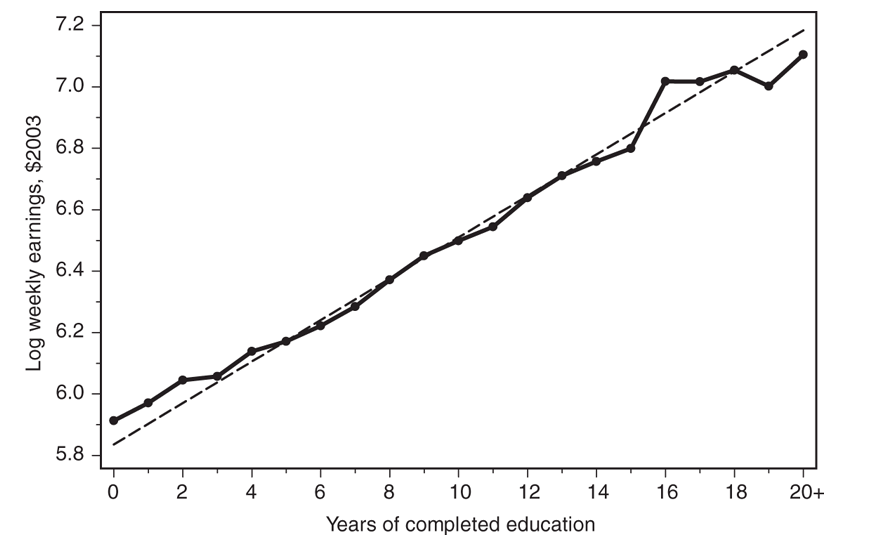
\includegraphics[scale=0.6]{educ_wages_linear.png}
\end{figure}
\end{frame}

\section{Finite Sample Properties OLS}

\begin{frame}
\frametitle{\: \: \: Unbiasedness} 
\toplinemedium
\begin{itemize}
\item Under strict exogeneity, $\mathbb{E}[\bm{u}|\bm{X}]=\bm{0}$, OLS/MM is unbiased:
\begin{eqnarray*}
\begin{array}{rl}
\bm{\hat{\beta}}^{ols}&=(\bm{X}^T \bm{X})^{-1} \bm{X}^T \bm{y} \\[1.2ex]
 \bm{\hat{\beta}}^{ols}  &=\bm{\beta}+(\bm{X}^T \bm{X})^{-1} \bm{X}^T \bm{u}  \\[1.2ex]
                                 \mathbb{E}[\bm{\hat{\beta}}^{ols}|\bm{X}] &=\bm{\beta}\underbrace{=}_{\text{by LIE}}  \mathbb{E}[\bm{\hat{\beta}}^{ols}]
\end{array}
\end{eqnarray*}
\item Pre-determinedness, $\mathbb{E}[u_i|x_{1i}, \cdot , x_{ki}]=0$, is not enough
\vspace{0.11in}
\item The linear CEF has to be correctly specified
\end{itemize}
\end{frame}


\begin{frame}
\frametitle{\: \: \: Variance under Spherical Errors} 
\toplinelarge
\begin{itemize}
\item Another important property of OLS is the conditional \textcolor{blue}{variance-covariance} matrix of estimates:
\begin{eqnarray*}
Var[\bm{\hat{\beta}}^{ols}|\bm{X}]=\mathbb{E}\left[(\bm{\hat{\beta}}^{ols}-\bm{\beta})(\bm{\hat{\beta}}^{ols}-\bm{\beta})^T \mathbb{|} \bm{X}\right]
\end{eqnarray*}
\item Assume that $\mathbb{E}\left[\bm{u}\bm{u}^T \mathbb{|} \bm{X}\right]=\sigma^2 \: \bm{I}$, then 
\begin{eqnarray*}
Var[\bm{\hat{\beta}}^{ols}|\bm{X}]=\sigma^2 (\bm{X}^T\bm{X})^{-1}
\end{eqnarray*}
\begin{itemize}
\item In practice, we estimate $\sigma^2$ by $\hat{\sigma}^2=\bm{\hat{u}}^T\bm{\hat{u}}(n-k)^{-1}$ 
\end{itemize}
\vspace{0.11in}
\item Spherical error terms is a very strict assumption, which is not usually satisfied, specially if the CEF is not linear
\vspace{0.11in}
\item  By the law of total variance, the unconditional variance is 
\begin{eqnarray*}
Var(\bm{\hat{\beta}}^{ols})=\sigma^2 \mathbb{E}[(\bm{X}^T\bm{X})^{-1}]
\end{eqnarray*}
\end{itemize}
\end{frame}



\begin{frame}
\frametitle{\: \: \: Distribution of regressors under Gauss-Markov} 
\toplinexlarge
\begin{itemize}
\item Classical or Gauss Markov Assumptions of Multiple Regression are:
\begin{enumerate}
\item If the population equation is given by (linear CEF) 
\begin{eqnarray*}
\bm{y}=\bm{X} \bm{\beta}+\bm{u}
\end{eqnarray*}
\item No perfect multicollinearity (i.e. $\bm{X}$ has full rank)
\vspace{0.11in}
\item Zero Conditional Mean (i.e. $E[\bm{u}|\bm{X}]=\bm{0}$)
\vspace{0.11in}
\item Homoskedasticity and no serial correlation (i.e. $Var[\bm{u}|\bm{X}]=\sigma^2 \: \bm{I}_{n}$)
\vspace{0.11in}
\item Population conditional error terms are jointly Normal: $\bm{u}|\bm{X}\sim N\left[\bm{0},\sigma^2 \: \bm{I}_N\right]$
\end{enumerate}
\item This yield the following result:
\begin{eqnarray*}
\bm{\hat{\beta}}|\bm{X}\sim N\left[\bm{\beta},\sigma^2 \: (\bm{X}^T\bm{X})^{-1}\right]
\end{eqnarray*}
\item Because of properties of the multivariate normal distribution, this yields the following marginal distribution of estimators:
\begin{eqnarray*}
\hat{\beta}_j|\bm{X}\sim N\left[\beta_j,\sigma^2 \: (\bm{X}^T\bm{X})_{jj}^{-1}\right]
\end{eqnarray*}
\end{itemize}
\end{frame}

\section{Asymptotic Properties OLS}

\begin{frame}
\frametitle{\: \: \: Consistency} 
\toplinesmall
\begin{itemize}
\item Classical Assumptions are very restrictive and not usually satisfied in practice
\vspace{0.11in}
\item  Therefore, modern econometrics relies on asymptotic properties of estimators, which are satisfied under weaker conditions 
\vspace{0.11in}
\item For instance, if we assume that $\mathbb{E}[\bm{X}_i^Tu_i]=\bm{0}$, then
\begin{eqnarray*}
\begin{array}{ll}
\underset{n\rightarrow \infty}{plim} \bm{\hat{\beta}}^{ols}  &=\underset{n\rightarrow \infty}{plim}\left[\bm{\beta}+(\frac{1}{n}\bm{X}^T \bm{X})^{-1} (\frac{1}{n}\bm{X}^T \bm{u}) \right] \\[1.4ex]
														         &=\bm{\beta}+ (\bm{S_{X^TX}})^{-1} \underset{n\rightarrow \infty}{plim}  (\frac{1}{n}\bm{X}^T \bm{u}) \\[1.4ex]
															&=\bm{\beta} \text{   (the OLS estimator is consistent)}
\end{array}
\end{eqnarray*}
\item Because we do not need mean independence, but zero covariance, the CEF does not need to be linear 
\vspace{0.11in}
\item Pre-determinedness is enough
\end{itemize}
\end{frame} 



\end{document}
